\documentclass[12pt, letterpaper]{article}
\usepackage{graphicx} % Required for inserting images
\setlength{\parskip}{.8em}
\setlength{\parindent}{2em}

\title{Credit Card Fraud Detection}
\author{Huy Pham}
\date{October 2024}
\begin{document}

\maketitle

\section{Introduction}
    \subsection{Project Motivation}
        In 2021, the Federal Trade Commission (FTC) received nearly 390,000 reports of credit card fraud, making it one of the most common types of fraud in the United States. This issue is projected to result in losses totaling \$165.1 billion over the next decade. Given the significant impact on society, leveraging machine learning technology to address this problem is increasingly beneficial.

    \subsection{Objective}
        In this project, our primary goal is to develop a reliable machine learning model to detect fraudulent credit card transactions. This involves a thorough analysis of the dataset to understand its distributions and engineering the most suitable model that captures the relationship between the target variable and features. We utilize Python libraries like Scikit-learn, Matplotlib, Numpy, and Pandas for implementation and visualization. The dataset used for this project was sourced from Kaggle. However, it is also important to note that this is an introductory project to machine learning which serves as an educational research project.
        
\section{Methodology}
    \subsection{Data Origin}
        The dataset was sourced from Kaggle, which was provided during a collaborative research project between Worldline and Machine Learning Group of ULB (Université Libre de Bruxelles) on big data mining and fraud detection.~\cite{Kaggle}
        
    \subsection{Data Understanding}
        The dataset provided has 31 predictors, which is quite time-consuming for the training process. Perhaps finding ways to reduce the dataset dimensions would benefit the project as well as the research model better.

        It seems that the dataset is sorted chronologically as the transactions happened as time went on. It is sensible to deem that the features ``Time'' and ``Amount'' are much less relevant to the desired model as frauds can happen at any time and any magnitude during the day. Furthermore, we want this research model of ours to be applicable to real world scenarios, which is not limited to the time frame this dataset was recorded from.

        It is also noted that PCA was performed on the dataset features due to privacy concerns, apart from these 3 features: ``Time'', ``Amount'', and ``Class''. Therefore, further consideration should be given to feature engineering to preserve the dataset's originality, methods like Standardization and Normalization might negatively impact the representation of the dataset.

        There are in total 284,807 transactions or data points in this dataset. It is also learned that the actual fraudulent transactions in this dataset is extremely underrepresented as the mean value for feature Class is extremely close to 0 (meaning there are a lot of 0s and very few 1s). The imbalance of the dataset is heavily concerning, as the relationship displayed in this dataset between the two classes are not so significant.

    \subsection{Data Preparation}
        The data types recorded in the dataset features are efficient for computing algorithms, which is beneficial to the training time of the research model. It is also noted that the dataset contains no invalid values (null values).

        Duplicates are identified within the dataset, with 1081 instances. However, dropping duplicates might impact the weight the duplicated points has on the dataset. In fact, the representation of positive class within the dataset is 0.173\% and after dropping the duplicates, the percentage goes down to 0.167\%. Even though the difference is negligible in most cases, it is still crucial to have more representation of these fraudulent data points in this extremely skewed dataset. This highlights the relevance of duplicated data points in the dataset to the relationship between two classes.
        
        \begin{figure}[h]
            \centering
            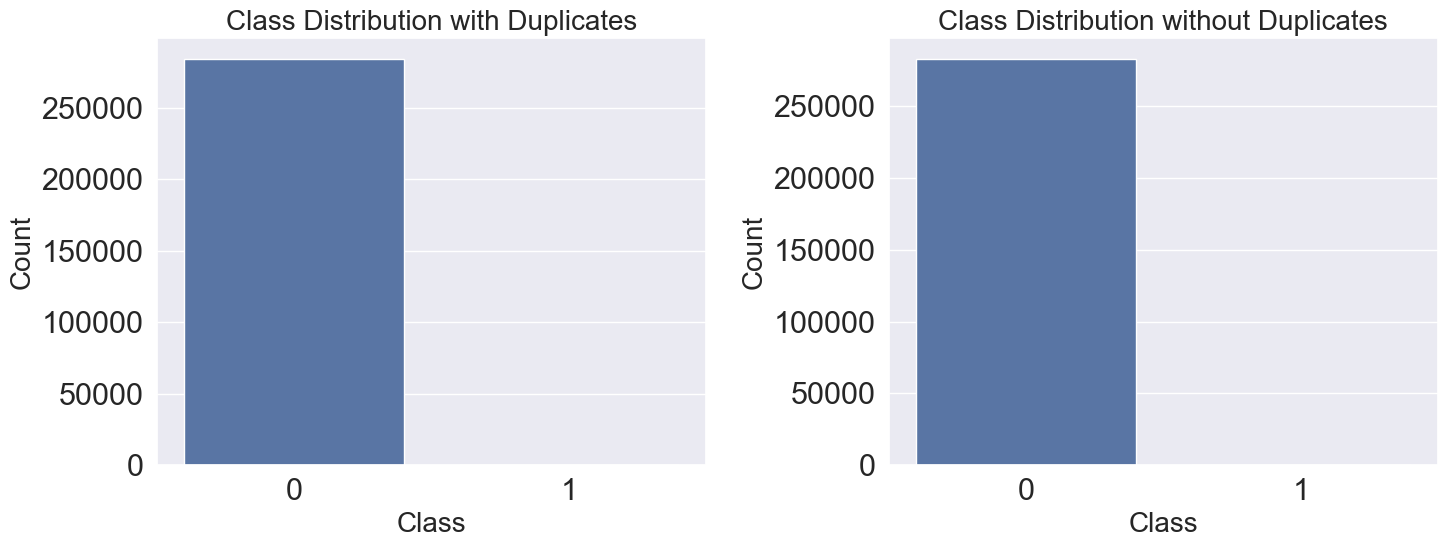
\includegraphics[width=1\linewidth]{Figures/Class-representation.png}
            \caption{Class Distributions Concerning Dataset Duplication}~\label{fig:enter-label}
        \end{figure}

    \subsection{Data Normalization \& Standardization}
        In order to ensure that the training data is 

    \subsection{Model Evaluation Metrics}
        Accuracy is highly a biased metric since the dataset is very skewed, other metrics may be more insightful in this case. Precision provides insights into how much of the model predictions for positive class (fraudulent) are true. On another hand, the Recall score stands for the model capability to identify the positive class given a test data.

        True Positive Rate and False Positive Rate are helpful to gain insights into how effective will the model be when deployed in real world. True Positive Rate (TPR) indicates how much of the actual positive class the model will identify. If TPR is high, the number of True Positive is significantly higher than the number of False Negative. False Positive Rate (FPR) conversely tells how much of the actual negative class the model will inaccurately identify. If the metric is high, the number of False Positive is significantly higher than the number of True Negative. In this case, we would want to maximize the TPR while keeping the FPR as low as possible.

        It should be noted that due to the imbalance in this dataset, the weight of the positive class is much heavier than that of the negative class. This means that TPR and FPR are implicitly affected, meaning that TPR is much harder to maximize and FPR is very likely to be small. Additionally, True Positives are considered to be much more important than True Negatives and False Negatives are much more important than False Positives. Due to these insights, additional metrics such as F-score and Precision-Recall AUC score are inquired.

        F-score is a particularly helpful metric, as it concerns the harmonic mean of Precision and Recall. This metric aims to favor those metrics being close to each other to achieve a high score. Considering the skewed interest between Precision and Recall, F2-score is selected to heighten the importance of Recall in this case.

        Precision-Recall AUC score is also considered in this project since it helps determine the better model given the imbalanced dataset. The better the score, the better the model is able to identify the True Positives without compromising Precision.

    \subsection{Research Models}
        In this introductory project, only two machine learning algorithms were suggested to classify the dataset, Logistic Regression and Random Forest.

        As per the Logistic Regression algorithm, this model assumes a linear relationship between the features and classes. This makes it quite hard to fit a training dataset that exhibits a non-linear relationship between the features and classes. On the other hand, Random Forest is able to learn a much more complex relationship that exists within a dataset. It is also noteworthy that while Logistic Regression is not flexible for many datasets, the model provides us with more precise control over the model fitting process. Depending on the relationship displayed within this research dataset, either a Logistic Regression or a Random Classifier can be the more optimal algorithm for this classification problem.
        
    \subsection{Bias and Variance}
        Bias and Variance are prevalent errors in machine learning models. In this case, due to the simplicity of Logistic Regression, it is bound to have high bias and low variance, resulting in an underfitting issue. This translates into our model performing poorly on both training and testing data. In contrast, Random Classifier has the ability to conform to the training data much better than Logistic Regression. This means that it can have low bias but high variance, meaning that the model performs well on the training dataset but poorly on the testing dataset.
        
        In order to prevent overfitting and underfitting, K-fold cross-validation is implemented to better gauge bias and variance in these research models. Although selecting a high number of folds for cross-validation ensures a more accurate interpretation of bias and variance, it also comes with a significant cost of extra computation. Therefore, the number of folds for cross-validation should depend on the available hardware to run these algorithms.
        
    \subsection{Class Imbalance}
        In order to improve the performance metrics of the models, handling the imbalance in the dataset is crucial to the project success. Ideally, research models should be better at identifying the positive class due to its underrepresentation. There are many popular approaches to this issue, such as class-weighting, SMOTE, and LDA.

        Class-weighting is considered in this project to counteract the imbalance in the dataset. This method directly affects the loss function of the models, putting much more emphasis on the positive class, thus favoring the detection of that class more. This can be an effective solution to this imbalanced dataset as we can fine-tune the weights to achieve desirable metrics.

        Synthetic Minority Over-sampling Technique (SMOTE) is a popular approach to handling imbalanced datasets. This approach specifically modifies the training dataset, synthetically creating more positive class data points by picking a middle point between two existing data points. However, this technique is prone to many issues as it depends on the original distribution of the minority class. If the distribution has many outliers, it will create more noise in the dataset. 
    
        Linear Discriminant Analysis (LDA) is another method often implemented for imbalanced datasets. This method reduces the dimension of the dataset, heightening the disparity of the classes. In this binary classification dataset, LDA will reduce the dataset down to a single dimension. This would be extremely beneficial to the models' fitting process as it would take much less time and, in theory, should improve the metrics.

        A mixed approach including all of these methods is also considered to achieve a better performing model.

        As mentioned earlier, PCA was performed on the dataset features, which might have negatively impacted the dataset's representation. Therefore, it is crucial to consider the impact of these methods on the dataset's originality.
        
\section{Results}
	We start by arbitrarily setting up the Logistic Regression and Random Forest models with parameters such that a normal fitting process would take 10--20 minutes. We also choose to use 10-fold cross-validation to evaluate the models.

    \subsection{Logistic Regression}
        The Logistic Regression model is configured as follows:
        \begin{itemize}
            \item Max\_iter: 5000
            \item Tol: 1e-3
            \item Random\_state: 9
        \end{itemize}
	    
        Max\_iter argument is set to 5000 to ensure that the model has enough time to converge to the optimal solution. The tolerance argument is set to 1e-3 to ensure that the model converges to the optimal solution within a reasonable margin of error. Random\_state is set to 9 to ensure that the model is reproducible.

        The model is trained on the training dataset and evaluated on the testing dataset. The model achieves the following metrics:
    
\section{Conclusion}
    
\begin{thebibliography} {1}
    \bibitem{Kaggle}
    Machine Learning Group---ULB.\@ “Credit Card Fraud Detection” Kaggle, 2018, www.kaggle.com/datasets/mlg-ulb/creditcardfraud.
    
\end{thebibliography}
    
\end{document}